\begin{frame}[t]{Definitions}
\begin{itemize}
\uncover<1->{\item The SAT Problem (\textbf{SAT}).}
\uncover<2->{\item Counting SAT Problem (\textbf{\#SAT}).}


\uncover<6->{\item Negation Normal Form (\textbf{NNF}).}
\uncover<7->{\item Conjunctive Normal Form (\textbf{CNF}).}
\uncover<8->{\item Decomposable Negation Normal Form (\textbf{DNNF}).}
\uncover<9->{\item deterministic Decomposable Negation Normal Form (\textbf{d-DNNF}).}
\uncover<10->{\item decision Decomposable Negation Normal Form (\textbf{dec-DNNF}).}
\end{itemize}

\only<1>{
\begin{block}{SAT}
\begin{itemize}
\item[--] Given a Boolean formula $\varphi$ of $n$ variables.
\item[?] Find an assignment that satisfies $\varphi$.
\end{itemize}
\end{block}
}

\only<2>{
\begin{block}{\#SAT}
\begin{itemize}
\item[--] Given a Boolean formula $\varphi$ of $n$ variables.
\item[?] How many assignments in $2^{\mathrm{Var}(\varphi)}$ satisfy $\varphi$?
\end{itemize}
\end{block}
}

\only<3-4>{
\begin{block}{Notation}
Let $\mathrm{SAT}(\chi) \subseteq 2^{\mathrm{VAR}(\chi)}$ be the set of all satisfying assignments of $\chi$
\vspace{-0.3cm}
$$\mathrm{SAT}(\chi) = \{\rho:\mathrm{VAR}(\chi) \rightarrow \{0, 1\} : \rho(\chi) = 1\}.$$
\vspace{-0.8cm}
\uncover<4->{$$\text{SAT: Is } \mathrm{SAT}(\varphi) = \emptyset.
\qquad \qquad \qquad
\text{\#SAT: Find } |\mathrm{SAT}(\varphi)|.$$}
\vspace{-0.6cm}
\end{block}
}

\only<5>{
\begin{block}{Example}
$$\varphi = X_1 \land (X_2 \lor \lnot X_3)$$
Clearly, \#SAT($\varphi$) = 3.
\end{block}
}

\only<6>{
\begin{block}{Negation Normal Form}
A Boolean formula $\varphi$ is in NNF form, if it contains only disjunctions and conjunctions over a set of positive and(or) negative literals.

\textbf{Example.} $\varphi = X_1 \lor \lnot X_2$.
\end{block}
}

\only<7>{
\begin{block}{Conjunctive Normal Form}
A Boolean formula $\varphi$ is in CNF, if it is a conjunction of one or more clauses, where each clauses is a disjunction of one or more literals. Note that each CNF formula is an NNF formula as well.
\end{block}
}

\only<8>{
\begin{block}{Decomposable Negation Normal Form}
A Boolean formula $\varphi$ is in DNNF, if it is in NNF and for each conjunction subformula $phi' := \psi_1 \land \psi_2$ we have $\mathrm{VAR}(\psi_1) \cap \mathrm{VAR}(\psi_2) = \emptyset$.
\end{block}
}

\only<9>{
\begin{block}{deterministic Decomposable Negation Normal Form}
A Boolean formula $\varphi$ is in d-DNNF, if it is in DNNF and for each disjunction subformula  $\varphi' = \psi_1 \lor \psi_2$ we have $\mathrm{SAT}(\psi_1) \cap \mathrm{SAT}(\psi_2) = \emptyset$.
\end{block}
}

\only<10->{
\begin{block}{decision Decomposable Negation Normal Form}
A Boolean formula $\varphi$ is in dec-DNNF, if it is in DNNF and each disjunction subformula  $\varphi'$ is of the form $\varphi' = (X \land \psi_1) \lor (\lnot X \land \psi_2)$ for some variable $X \in \mathrm{VAR}(\varphi)$.

\uncover<11>{\textbf{Note.} Each dec-DNNF is a d-DNNF.}
\end{block}
}
\end{frame}

\begin{frame}[t]{Assignments}
	\begin{itemize}[<+->]
		\item Given a CNF Formula $\varphi$, an \textbf{assignment} for $C$ is a function $\tau : \mathrm{VAR}(C) \rightarrow \{0, 1\}$.
		\item For $V' \subseteq \mathrm{VAR}(C)$, we define the \textbf{partial assignment} $\tau_{|V'} : V' \rightarrow \{0, 1\}$ as $\tau$ restricted to the variables in $V'$.
		\item A partial assignment $\tau_{|V'}$ satisfies a CNF-formula $\varphi$ ($\tau_{|V'} \models \varphi$), if for each clause $C \in \varphi$ there is a variable $v \in \mathrm{VAR}(C) \cap V'$ such that $\tau_{|V'}(v) = 1$ if and only if $v$ appears in $C$ as a positive literal.

	\end{itemize}
	\uncover<4>{
	\begin{block}{Example}
		$$\varphi := (v_1 \lor \lnot v_2 \lor v_3) \land (v_1 lor v_2) \land (\lnot v2 \lor \lnot v_3)$$
		For $V' = \{v_1, v_2\}, \tau_{|V'}(v_1) = 1, \tau_{|v'}(v_2) = 0$,
		the partial assignment $\tau_{|V'}$ satisfies $\varphi$.
	\end{block}
	}
\end{frame}

\begin{frame}[t]{Structuredness of a formula}
	\begin{itemize}[<+->]
		\item Let $\varphi$ be a DNNF formula and let $V := \mathrm{VAR}(\varphi)$.
		\item A \textbf{$\mathbf{v}$Tree} $T$ is a binary tree where the leaves of the tree has a one-to-one correspondence to the variables of $\varphi$.
		\item The formula $\varphi$ respects $T$ if and only if for each subformula of  $\varphi$ of the form $\varphi' := \psi_1 \land \psi_2$, there is a vertex $v \in V(T)$ with two children $v_1, v_2$, where $\mathrm{VAR}(\psi_1)\subseteq V(T_{v_1})$ and $\mathrm{VAR}(\psi_2) \subseteq V(T_{v_2})$, where $T_v$ is the subtree of $T$ rooted at $v$. We say $\varphi'$ respects $v$ in this case.
		\item A formula $\varphi$ is structured, if there is a $v$tree $T$ over the vertices of $\varphi$, such that $\varphi$ respects $T$.
	\end{itemize}

	\uncover<3->{
	\begin{minipage}{.49\linewidth}
		$$(x\land(y\lor z)) \lor (z \textcolor{red}{\bm{\land}} \lnot x)$$
	\end{minipage}
	\hfill
	\begin{minipage}{.49\linewidth}
		\centering
		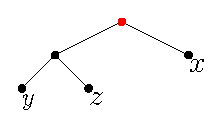
\includegraphics[width=.6\linewidth]{figures/vtree.eps}
	\end{minipage}
	}
\end{frame}

\begin{frame}[t]{Hypergraphs and $\beta$-acyclic graphs}
	\begin{minipage}{.59\linewidth}
	\begin{itemize}
		\item Hypergraphs $\mathcal{G}$.
			\begin{itemize}
				\item A set of vertices $V(\mathcal{G})$.
				\item Edges $E(\mathcal{G})$, defined as 
				\item[] subsets over $V(\mathcal{G})$.
			\end{itemize}
		\item Different ways to translate
		\item[] \hspace{1cm} to hypergraphs.
		\item $\beta$ acyaclic hypergraphs.
			\begin{itemize}
				\item Defined on the edges.
				\item Let $\rho := v_1, \dots v_n$ be an
				\item[] \hspace{1cm}enumeration of the vertices.
				\item $\rho$ is an $\beta$-elimination, if for all
				\item[] \hspace{1cm}$e_1, e_2 \in E(\mathcal{G})$ and $v_i \in e_1 \cap e_2$,
				\item[]\hspace{1cm}$e_{1|\geq i} \subseteq e_2$ or $e_{2|\geq i} \subseteq e_1$.
				\item A hypergraph is $\beta$-acyclic,
				\item[] \hspace{1cm} if it admits an elimination.

			\end{itemize}
	\end{itemize}
\end{minipage}
\begin{minipage}{.39\linewidth}
\centering
\begin{tikzpicture}
    \node (v1) at (1,2) {};
    \node (v2) at (1.5,3) {};
    \node (v3) at (4,2.5) {};
    \node (v4) at (2,1) {};
    \node (v5) at (3.5,0.5) {};

    \begin{scope}[fill opacity=0.8]
    \filldraw[fill=yellow!50] ($(v1)+(-0.5,0)$) 
        to[out=90,in=180] ($(v2) + (0,0.5)$) 
        to[out=0,in=90] ($(v3) + (1,0)$)
        to[out=270,in=0] ($(v2) + (1,-0.8)$)
        to[out=180,in=270] ($(v1)+(-0.5,0)$);
    \filldraw[fill=blue!70] ($(v4)+(-0.5,0.2)$)
        to[out=90,in=180] ($(v4)+(0,1)$)
        to[out=0,in=90] ($(v4)+(0.6,0.3)$)
        to[out=270,in=0] ($(v4)+(0,-0.6)$)
        to[out=180,in=270] ($(v4)+(-0.5,0.2)$);

    \filldraw[fill=green!80] ($(v3)+(-0.5,-0.2)$) 
        to[out=90,in=180] ($(v3) + (0.2,0.4)$) 
        to[out=0,in=90] ($(v5) + (0.3,-0.1)$)
        to[out=270,in=0] ($(v5) + (0,-0.3)$)
        to[out=180,in=270] ($(v3)+(-0.5,-0.2)$);

    \filldraw[fill=red!40] ($(v2)+(-0.5,-0.2)$) 
        to[out=90,in=180] ($(v2) + (0.2,0.4)$) 
        to[out=0,in=180] ($(v3) + (0,0.3)$)
        to[out=0,in=90] ($(v3) + (0.3,-0.1)$)
        to[out=270,in=0] ($(v3) + (0,-0.3)$)
        to[out=180,in=0] ($(v3) + (-1.3,0)$)
        to[out=180,in=270] ($(v2)+(-0.5,-0.2)$);
    \end{scope}

    \foreach \v in {1,2,...,5} {
        \fill (v\v) circle (0.1);
    }

    \fill (v1) circle (0.1) node [right] {$v_1$};
    \fill (v2) circle (0.1) node [below left] {$v_2$};
    \fill (v3) circle (0.1) node [left] {$v_3$};
    \fill (v4) circle (0.1) node [right] {$v_4$};
    \fill (v5) circle (0.1) node [above] {$v_5$};

    \node at (3.8,3.2) {$e_1$};
    \node at (2.3,3) {$e_2$};
    \node at (3.8,1.5) {$e_3$};
    \node at (2, 1.5) {$e_4$};
\end{tikzpicture}

\end{minipage}
\footnotetext[1]{$e_{|\geq i} := e \cap \{v_i, \dots v_n\}$.}
\end{frame}

\begin{frame}[t]{Incidence graphs and structure of formulas}
	\begin{itemize}
		\item The \textbf{incidence graph} of $\mathcal{G}$ is a 
		\item[] \hspace{1cm}bipartite graph $(V(\mathcal{G}) \cup E(\mathcal{G}), E)$
		\item[] \hspace{1cm},where $\{v, e\} \in E$ iff $v \in e$.
			\vspace{.5cm}
		\item Hypergraph of a CNF-Formula.
		\item The incidence graph of a CNF-Formula is 
		\item[] \hspace {1cm} the incidence graph of its hyper graph.
		\item A CNF-Formula is $\beta$-acyclic if its hypergraph is.
	\end{itemize}

\end{frame}
	

